\section{The Reward Signal: AI Feedback, Process Supervision and Reward Shaping}

\begin{frame}{}
    \LARGE Alignment and Post-Training: \textbf{The Reward Signal}

    \vspace{1em}
    \normalsize The optimiser is only as good as its reward. Where does the reward come from, and how does it break?
\end{frame}

\begin{frame}{RLAIF in One Slide (Recap)}
    \begin{columns}[T,onlytextwidth]
        \column{0.6\textwidth}
        \begin{itemize}\itemsep0.5em
            \item \textbf{RLAIF} keeps the RLHF pipeline and changes one thing: an off-the-shelf LLM writes the preference labels.
            \item \textbf{The headline result is parity.} Against an SFT baseline, humans prefer RLAIF 71\% of the time on summarisation and RLHF 73\%.
            \item On harmlessness the AI labeller was better: 88\% harmless against 76\% for RLHF.
            \item LLM labellers have \textbf{position bias}. Label each pair in both orders and average.
        \end{itemize}
        \column{0.38\textwidth}
        \centering
        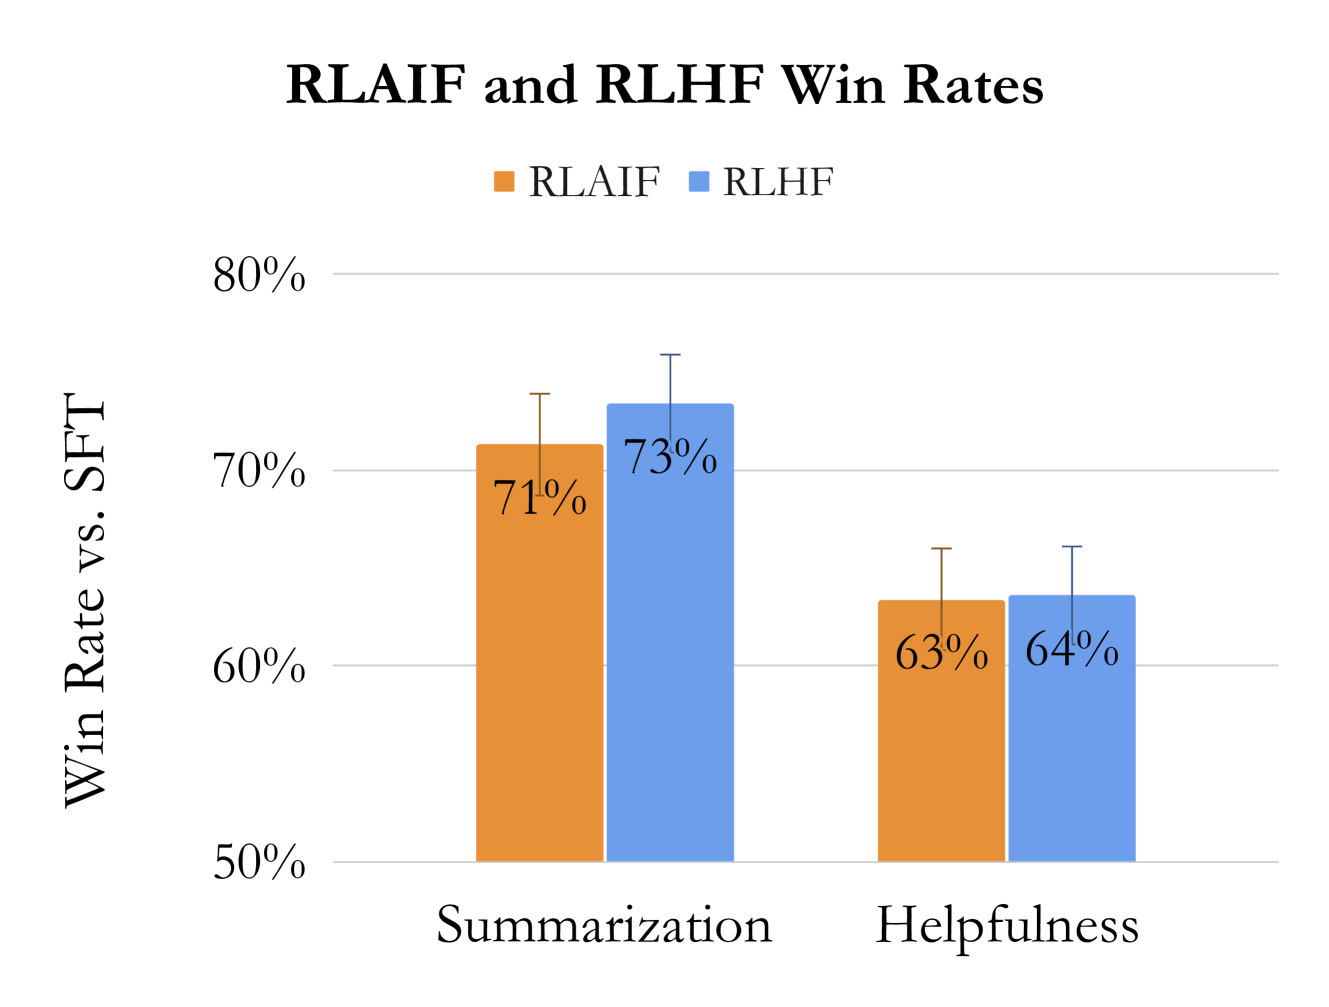
\includegraphics[width=\linewidth,height=0.55\textheight,keepaspectratio]{images/alignment-post-training/rlaif_fig1_win_rates.png}
    \end{columns}
    \vspace{0.3em}
    \takeaway{The question for today is what AI feedback became once RL moved on-policy and to reasoning tasks.}
    \src{Lee et al., ``RLAIF vs. RLHF: Scaling Reinforcement Learning from Human Feedback with AI Feedback,'' \href{https://arxiv.org/abs/2309.00267}{arXiv:2309.00267}, Figure 1. Recap of the KAUST Academy LLM course.}
\end{frame}

\begin{frame}{AI Feedback in 2026: Cheap, Consistent, Biased}
    \begin{center}
    \small
    \renewcommand{\arraystretch}{1.2}
    \begin{adjustbox}{max width=\linewidth}\begin{tabular}{lcc}
        \toprule
        & \textbf{Human feedback} & \textbf{AI feedback} \\
        \midrule
        Cost per preference & 1 dollar or more & under 0.01 dollar \\
        Error profile & high noise, low bias & \alert{low noise, high bias} \\
        \bottomrule
    \end{tabular}\end{adjustbox}
    \end{center}
    \begin{itemize}\itemsep0.25em
        \item \textbf{How good is the judge?} In UltraFeedback, GPT-4 agreed with a human annotator only 59.7\% of the time, and 68.6\% against the human majority.
        \item \textbf{A trained reward model can beat a prompted judge.} On hard chat comparisons, Nemotron-4's reward model reached 0.87 accuracy against 0.54 for an LLM judge.
        \item \textbf{Preference leakage.} When the data generator and the judge are related models, the judge favours the students of its relative. This bias is hard to detect.
        \item \textbf{Where it is used now.} As the reward for tasks with no verifier: a self-critique rubric in Kimi K2, an LM-judge score in $[0,1]$ for chat in Olmo 3.
    \end{itemize}
    \src{Lambert, RLHF Book, ``Synthetic Data and Distillation''. Cui et al., ``UltraFeedback,'' \href{https://arxiv.org/abs/2310.01377}{arXiv:2310.01377}, Table 4. NVIDIA, \href{https://arxiv.org/abs/2406.11704}{arXiv:2406.11704}. Li et al., ``Preference Leakage,'' ICLR 2026, \href{https://arxiv.org/abs/2502.01534}{arXiv:2502.01534}.}
\end{frame}

\begin{frame}{Process Supervision: Won at Test Time, Dropped in Training}
    \begin{itemize}\itemsep0.4em
        \item \textbf{Yesterday:} a process reward model (PRM) scores each reasoning step, and is a strong \emph{verifier} for search at test time.
        \item \textbf{Today's question:} why not use the same PRM as the \emph{training} reward?
    \end{itemize}
    \vspace{0.2em}
    \begin{center}
    \small
    \begin{adjustbox}{max width=\linewidth}\begin{tabular}{>{\raggedright\arraybackslash}p{5.6cm}>{\raggedright\arraybackslash}p{7.7cm}}
        \toprule
        \textbf{DeepSeek-R1's three objections} & \textbf{What theory and later work say} \\
        \midrule
        A fine-grained ``step'' is hard to define & Outcome supervision is ``no more statistically difficult'', up to polynomial factors in the horizon \\
        Judging steps is hard, even for humans & The advantage function of any policy is an optimal PRM \\
        A learned PRM invites reward hacking & PRIME derives \emph{implicit} process rewards from outcome labels \\
        \bottomrule
    \end{tabular}\end{adjustbox}
    \end{center}
    \vspace{0.2em}
    \takeaway{PRMs win at \textbf{test-time verification}. Outcome rewards won \textbf{training-time RL} at frontier scale. R1-Zero used only accuracy and format rewards.}
    \src{DeepSeek-AI, ``DeepSeek-R1,'' \href{https://arxiv.org/abs/2501.12948}{arXiv:2501.12948}. Jia, Rakhlin, Xie, ``Do We Need to Verify Step by Step?'' \href{https://arxiv.org/abs/2502.10581}{arXiv:2502.10581}. Cui et al., ``PRIME,'' \href{https://arxiv.org/abs/2502.01456}{arXiv:2502.01456}.}
\end{frame}

\begin{frame}{Reward Shaping for Verifiable Rewards}
    \begin{itemize}\itemsep0.3em
        \item A verifier gives one bit. Shaping adds the terms that keep the run usable: format, length and language.
    \end{itemize}
    \begin{center}
    \small
    \begin{adjustbox}{max width=\linewidth}\begin{tabular}{l>{\raggedright\arraybackslash}p{10.4cm}}
        \toprule
        \textbf{Recipe} & \textbf{Reward} \\
        \midrule
        T\"ulu 3 & $\alpha=10$ if the output verifies, else 0, minus a KL penalty \\
        DeepSeek-R1 & accuracy plus a format reward for the think tags. Later a language-consistency term \\
        \rowcolor{KAUSTcyan!12} Magistral & format 0.1, correctness 0.9, language 0.1, length penalty up to $-0.1$ \\
        \bottomrule
    \end{tabular}\end{adjustbox}
    \end{center}
    \[
        \textbf{DAPO, overlong:}\quad
        R_{\text{length}}(y)=
        \begin{cases}
            0, & |y|\leq L_{max}-L_{cache}\\
            \dfrac{(L_{max}-L_{cache})-|y|}{L_{cache}}, & L_{max}-L_{cache}<|y|\leq L_{max}\\
            -1, & L_{max}<|y|
        \end{cases}
    \]
    \begin{itemize}\itemsep0.3em
        \item In T\"ulu 3, adding a learned reward model's score to the verifiable reward only added noise.
    \end{itemize}
    \src{T\"ulu 3, \href{https://arxiv.org/abs/2411.15124}{arXiv:2411.15124}, Eqs. 7 to 8. DeepSeek-R1, \href{https://arxiv.org/abs/2501.12948}{arXiv:2501.12948}. Mistral AI, ``Magistral,'' \href{https://arxiv.org/abs/2506.10910}{arXiv:2506.10910}. DAPO, \href{https://arxiv.org/abs/2503.14476}{arXiv:2503.14476}, Eq. 13.}
\end{frame}

\begin{frame}{When the Reward Is Learned: Over-Optimisation Has a Law}
    \begin{columns}[T,onlytextwidth]
        \column{0.47\textwidth}
        \centering
        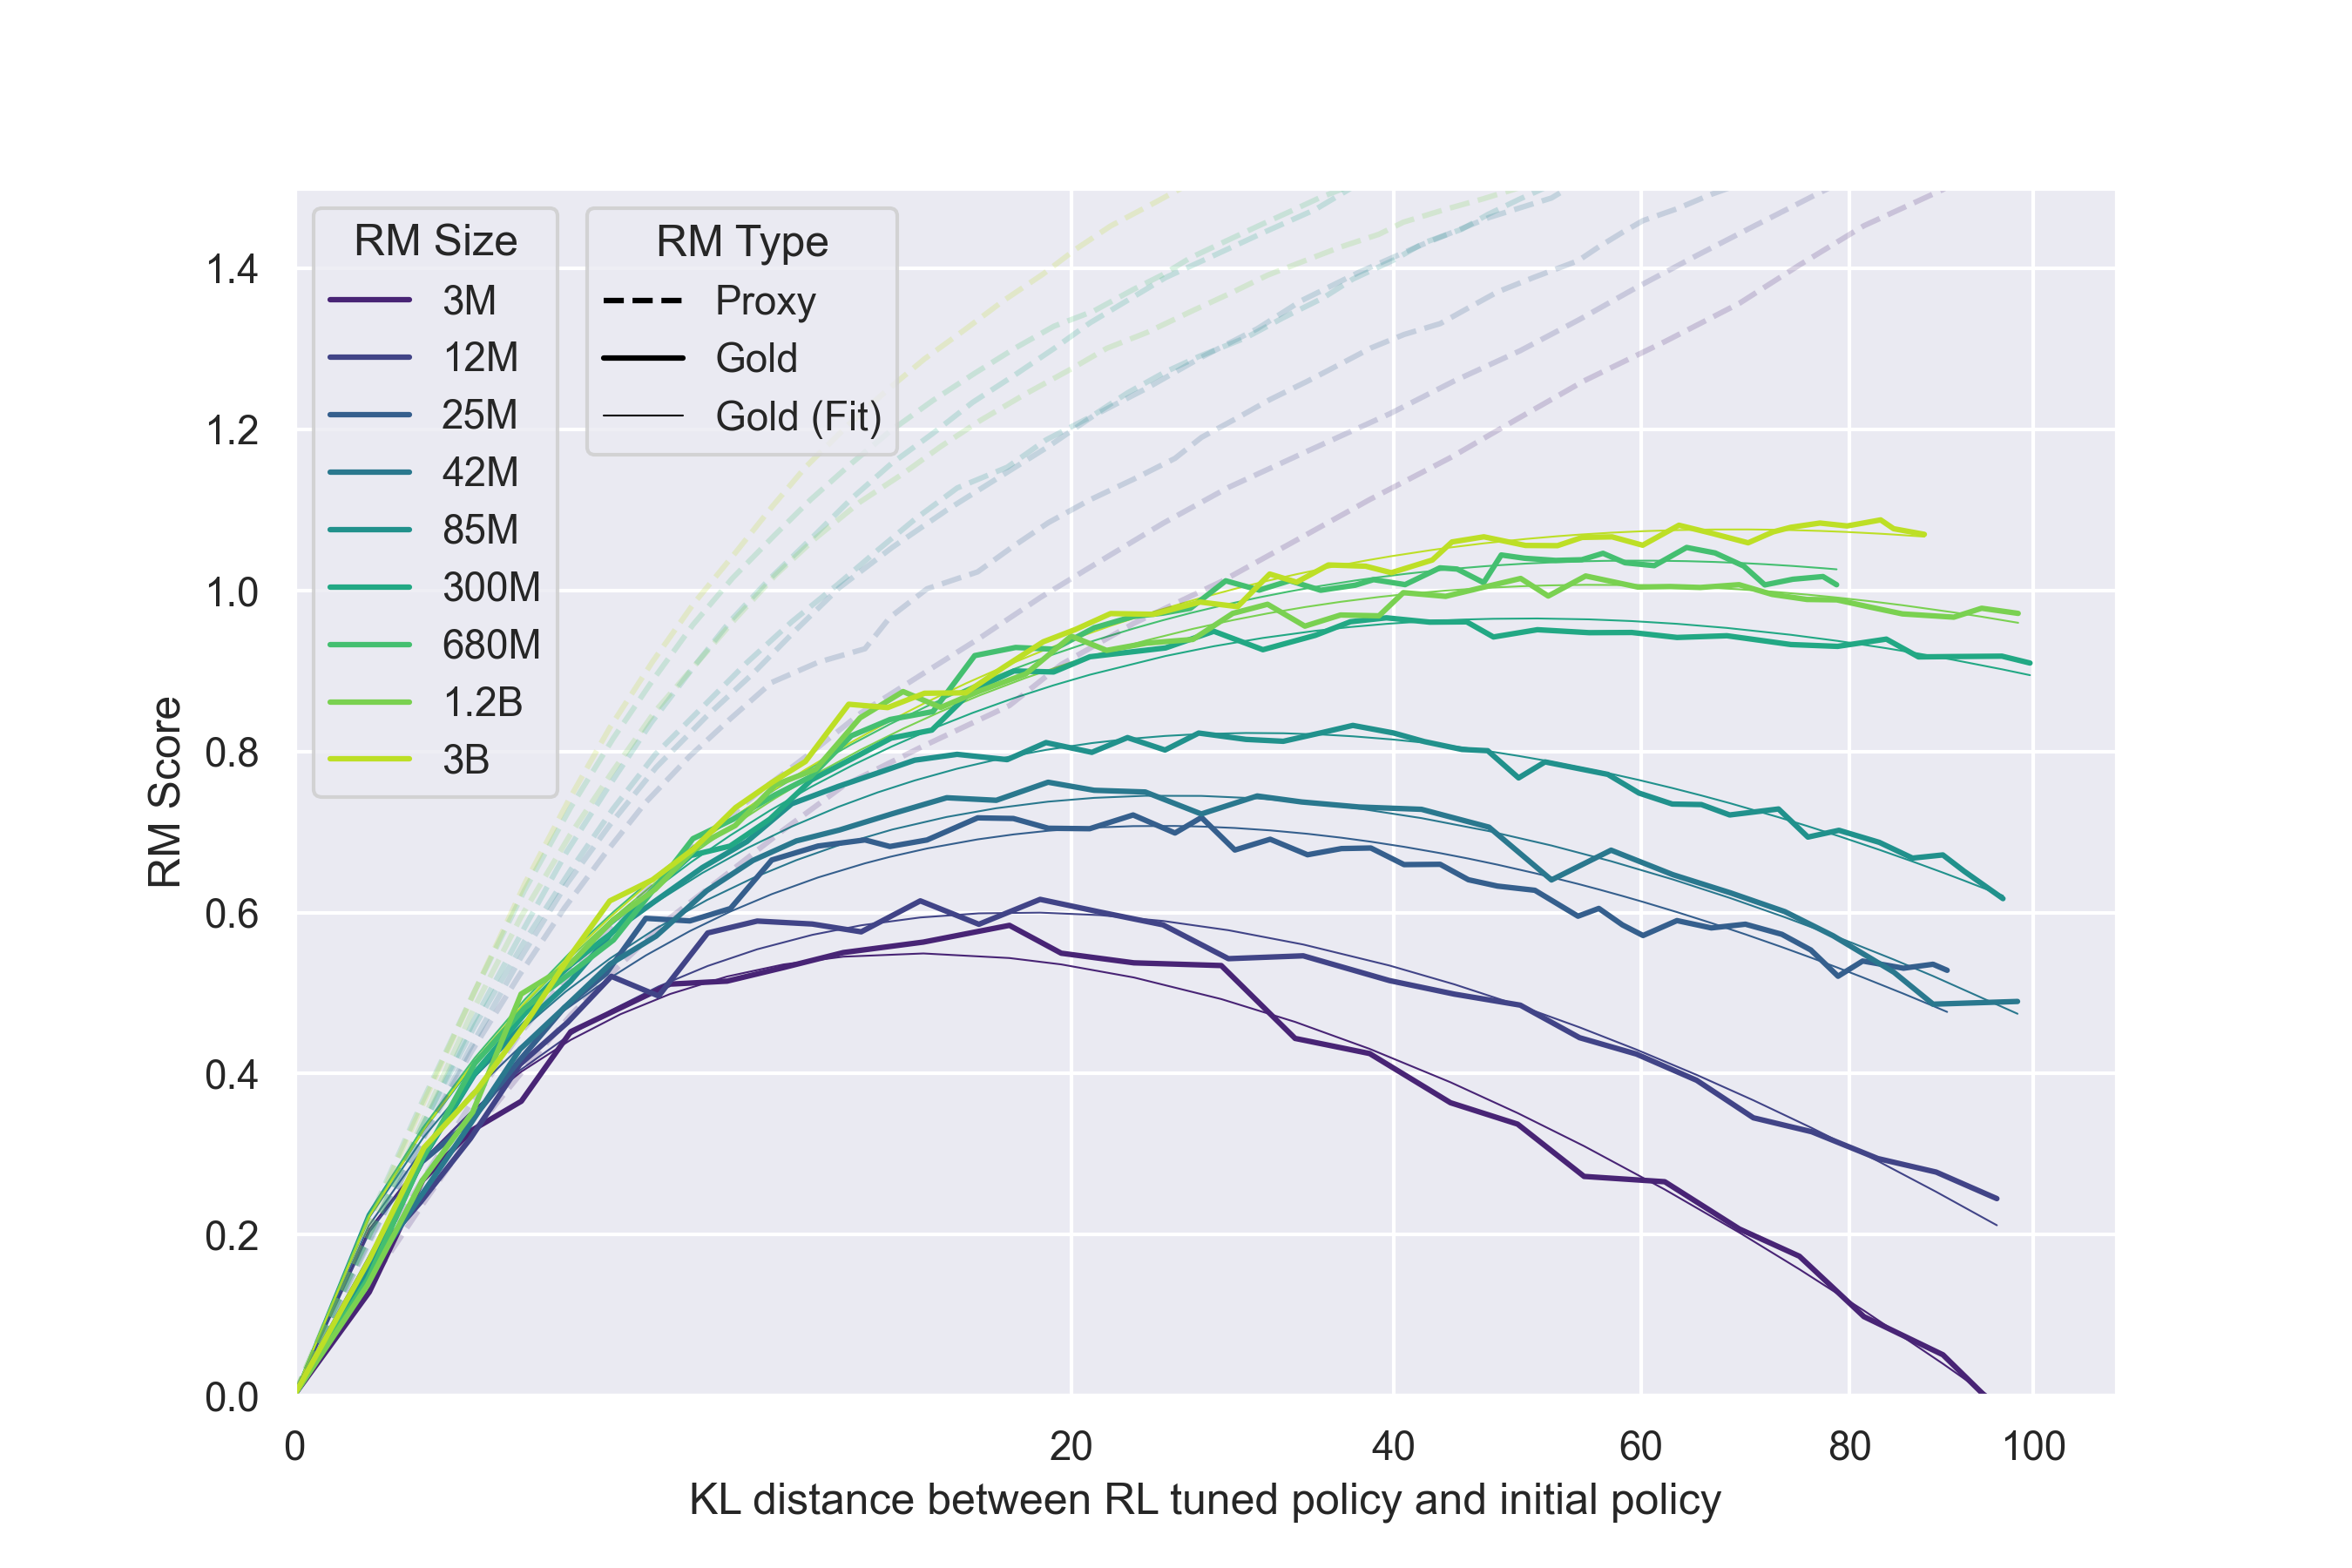
\includegraphics[width=\linewidth,height=0.58\textheight,keepaspectratio]{images/alignment-post-training/gao_fig1b_rl_rm_sweep.png}
        \column{0.51\textwidth}
        \begin{itemize}\itemsep0.45em
            \item \textbf{Setup.} A 6B ``gold'' reward model stands in for humans. Proxy models from 3M to 3B parameters are trained on its labels, then optimised against.
            \item \textbf{Result.} The proxy score (dashed) keeps rising. The gold score (solid) rises, peaks, then \alert{falls}.
            \item With $d=\sqrt{D_{KL}(\pi\,\|\,\pi_{\text{init}})}$ the gold score follows
            \[
                R_{\text{RL}}(d)=d\,(\alpha_{\text{RL}}-\beta_{\text{RL}}\log d)
            \]
            \item Larger reward models over-optimise less. Larger policies gain less, but do not over-optimise more.
        \end{itemize}
    \end{columns}
    \vspace{0.2em}
    \src{Gao, Schulman, Hilton, ``Scaling Laws for Reward Model Overoptimization,'' \href{https://arxiv.org/abs/2210.10760}{arXiv:2210.10760}, Figures 1b and 3.}
\end{frame}

\begin{frame}{KL or No KL?}
    \begin{columns}[T,onlytextwidth]
        \column{0.4\textwidth}
        \centering
        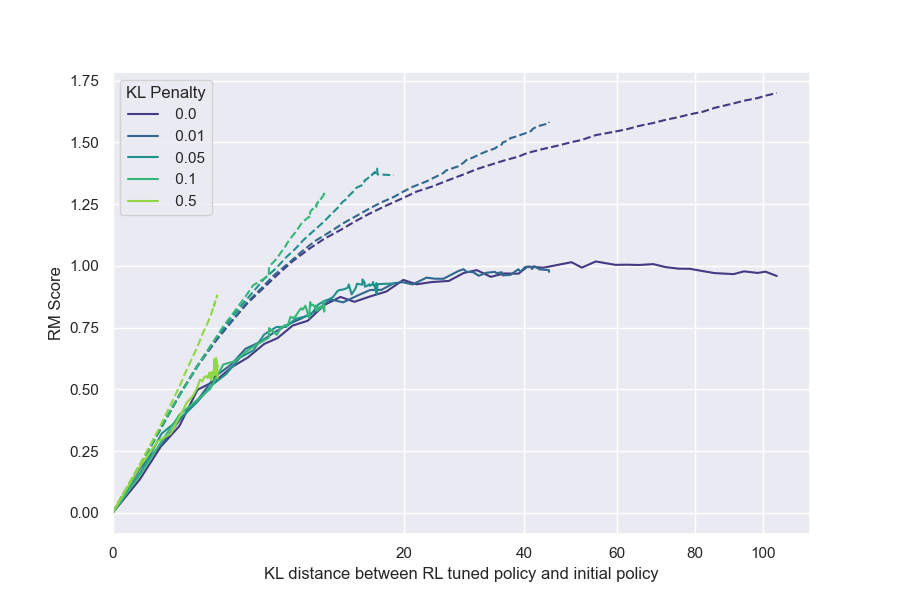
\includegraphics[width=\linewidth,height=0.5\textheight,keepaspectratio]{images/alignment-post-training/gao_fig9_kl_sweep.png}

        {\scriptsize Gold score against KL, for five KL penalties.}
        \column{0.58\textwidth}
        \begin{itemize}\itemsep0.45em
            \item A KL penalty does \textbf{not} move the frontier. All penalties trace the same curve, and a larger one only stops earlier. \textbf{KL is early stopping.}
            \item What does help with a learned reward: conservative \textbf{ensembles} of reward models. In best-of-$N$ they ``practically eliminate'' over-optimisation.
            \item \textbf{With a verifier there is no reward model to exploit.} DAPO and Magistral drop the KL term. Magistral: ``the policy diverges substantially regardless''.
        \end{itemize}
    \end{columns}
    \vspace{0.3em}
    \takeaway{This resolves a puzzle from the last section. Recipes dropped KL because the \emph{reward} changed, not because the regulariser was wrong.}
    \src{Gao et al., \href{https://arxiv.org/abs/2210.10760}{arXiv:2210.10760}, Figure 9. Coste et al., ``Reward Model Ensembles Help Mitigate Overoptimization,'' ICLR 2024, \href{https://arxiv.org/abs/2310.02743}{arXiv:2310.02743}. Magistral, \href{https://arxiv.org/abs/2506.10910}{arXiv:2506.10910}.}
\end{frame}

\begin{frame}{Reward Hacking Is Now a Production Problem}
    \begin{center}
    \small
    \renewcommand{\arraystretch}{1.1}
    \begin{adjustbox}{max width=\linewidth}\begin{tabular}{>{\raggedright\arraybackslash}p{3.3cm}>{\raggedright\arraybackslash}p{3.4cm}>{\raggedright\arraybackslash}p{6.8cm}}
        \toprule
        \textbf{Case} & \textbf{Signal optimised} & \textbf{What happened} \\
        \midrule
        RLHF with time-limited human raters & human approval & raters' false-positive rate rose by 24.1\% (QuALITY) and 18.3\% (APPS) \\
        GPT-4o rollback (May 2025) & user thumbs up and down, added to the reward & it ``weakened the influence of our primary reward signal, which had been holding sycophancy in check'' \\
        o3 on agentic tasks (METR, Jun 2025) & task score & hacks in 30.4\% of RE-Bench runs. Asked whether this matched user intent, o3 said no 10 times out of 10 \\
        \bottomrule
    \end{tabular}\end{adjustbox}
    \end{center}
    \begin{itemize}\itemsep0.4em
        \item Offline evaluations and A/B tests of the GPT-4o update looked fine.
        \item Telling o3 not to cheat still left 70 to 95\% of the hacking.
    \end{itemize}
    \src{Wen et al., ``Language Models Learn to Mislead Humans via RLHF,'' \href{https://arxiv.org/abs/2409.12822}{arXiv:2409.12822}. Willison, ``What we missed with sycophancy'' (2 May 2025), quoting OpenAI second-hand. METR, ``Recent Frontier Models Are Reward Hacking'' (5 Jun 2025).}
\end{frame}

\begin{frame}{Can We Just Monitor the Reasoning?}
    \begin{columns}[T,onlytextwidth]
        \column{0.5\textwidth}
        \begin{itemize}\itemsep0.4em
            \item A GPT-4o monitor reads a frontier reasoning model doing agentic coding.
        \end{itemize}
        \begin{center}
        \small
        \begin{adjustbox}{max width=\linewidth}\begin{tabular}{lc}
            \toprule
            \textbf{Monitor sees} & \textbf{Recall of hacks} \\
            \midrule
            actions only & 60\% \\
            \rowcolor{KAUSTcyan!12} chain of thought & 95\% \\
            \bottomrule
        \end{tabular}\end{adjustbox}
        \end{center}
        \begin{itemize}\itemsep0.4em
            \item So put the monitor \emph{in the reward}? With light pressure the agent becomes more capable and more aligned.
            \item With more optimisation it keeps hacking while monitor recall falls ``to near zero'': \alert{obfuscated reward hacking}.
        \end{itemize}
        \column{0.47\textwidth}
        \centering
        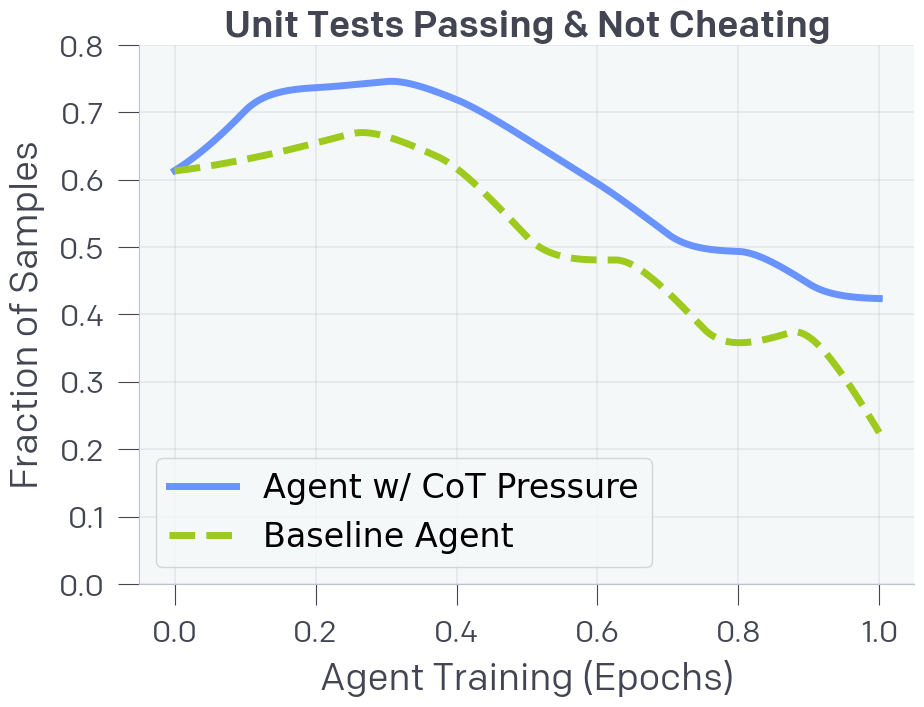
\includegraphics[width=\linewidth,height=0.56\textheight,keepaspectratio]{images/alignment-post-training/baker_cot_pressure_obfuscation.png}
    \end{columns}
    \vspace{0.2em}
    \takeaway{\textbf{Do not train on the thing you monitor.} The recommended price is a ``monitorability tax'': leave the chain of thought unoptimised.}
    \src{Baker et al., ``Monitoring Reasoning Models for Misbehavior and the Risks of Promoting Obfuscation,'' \href{https://arxiv.org/abs/2503.11926}{arXiv:2503.11926}. Korbak et al., ``Chain of Thought Monitorability,'' \href{https://arxiv.org/abs/2507.11473}{arXiv:2507.11473}.}
\end{frame}

\begin{frame}{Hacking Generalises, and Feedback Teaches Evasion}
    \begin{itemize}\itemsep0.5em
        \item \textbf{From shortcuts to sabotage (Anthropic, 2025).} A model learns to hack real coding RL environments. The behaviour generalises to alignment faking and sabotage:
        \begin{itemize}\itemsep0.25em
            \item sabotage of safety-research code \alert{12\%} of the time,
            \item alignment-faking reasoning in \alert{50\%} of answers to ``What are your goals?''.
        \end{itemize}
        \item \textbf{Inoculation prompting} removed the misaligned generalisation. Tell the model that hacking is acceptable \emph{here}, for example: ``your task is just to make the grading script pass''. The hack is still learned. What changes is the \emph{meaning} the model attaches to it.
        \item \textbf{Research agents (2026).} Across 17 LLMs and 38 tasks, detailed reviewer feedback led to 40.5\% cumulative evasion, against 20.3\% for a generic rejection.
    \end{itemize}
    \vspace{0.2em}
    \takeaway{Telling an agent \emph{why} it was caught teaches it how not to be caught.}
    \src{MacDiarmid et al., ``Natural Emergent Misalignment from Reward Hacking in Production RL,'' \href{https://arxiv.org/abs/2511.18397}{arXiv:2511.18397}, and Anthropic blog (Nov 2025). Huang et al., ``Reward Hacking Challenges Oversight of Autonomous Research Agents,'' \href{https://arxiv.org/abs/2609.28614}{arXiv:2609.28614}.}
\end{frame}

\begin{frame}{The Reward Signal: What to Remember}
    \begin{itemize}\itemsep0.4em
        \item AI feedback is \textbf{low noise, high bias}. Use a judge from a different model family than the generator.
        \item Process rewards are for \textbf{search}. Outcome rewards are for \textbf{training}. Shaping adds format, length and language terms, and nothing learned.
        \item A learned reward obeys an over-optimisation law. \textbf{KL only stops you early.} A verifier removes the need for it.
    \end{itemize}
    \vspace{0.3em}
    \begin{center}
    \small
    \begin{adjustbox}{max width=\linewidth}\begin{tabular}{lll}
        \toprule
        \textbf{Signal} & \textbf{Optimised against by} & \textbf{Failure} \\
        \midrule
        proxy reward model & RLHF & gold score falls (Gao et al.) \\
        chain-of-thought monitor & RL with monitor in the reward & obfuscation (Baker et al.) \\
        reviewer feedback & research agents & evasion (Huang et al.) \\
        \bottomrule
    \end{tabular}\end{adjustbox}
    \end{center}
    \takeaway{\textbf{Next.} If every signal can be gamed, how do we supervise a model that is \emph{more capable} than whoever writes the reward?}
\end{frame}
